
\documentclass[acmlarge,nonacm=true]{acmart}
\usepackage{adjustbox}
\usepackage{multirow}
\usepackage{graphicx}
\usepackage{afterpage}
\usepackage{subcaption}

\newcommand\blankpage{%
	\null
	\thispagestyle{empty}%
	\addtocounter{page}{-1}%
	\newpage}

%%
%% \BibTeX command to typeset BibTeX logo in the docs
\AtBeginDocument{%
  \providecommand\BibTeX{{%
    \normalfont B\kern-0.5em{\scshape i\kern-0.25em b}\kern-0.8em\TeX}}}


\begin{document}
	
	\begin{titlepage}
		\begin{center}
			\vspace*{1cm}
			
\includegraphics[width=0.7\textwidth]{fig/ntu_logo}
			\vspace{0.8cm}
			\linebreak
			\Huge
			\textbf{Experiment 1: Parametric Curves}
			
			\vspace{0.5cm}
			\LARGE
			CZ2003 Computer Graphics and Visualization
			
			\vspace{1.5cm}
			\textbf{SS3}\\
			
			\begin{table}[h]
				\begin{tabular}{lc}
					Name & Matric Number \\\hline
					Pang Yu Shao & U1721680D \\
				\end{tabular}
			\end{table}
			
			
			
			\vfill
			
			\vspace{0.8cm}
			
			
			
			\Large
			SCHOOL OF COMPUTER SCIENCE AND ENGINEERING\\
			NANYANG TECHNOLOGICAL UNIVERSITY\\
			SINGAPORE\\
			2nd Febraury 2021
			
		\end{center}
	\end{titlepage}

 

%%
%% The "title" command has an optional parameter,
%% allowing the author to define a "short title" to be used in page headers.
\title{CZ2003 Computer Graphics and Visualization}

%%
%% The "author" command and its associated commands are used to define
%% the authors and their affiliations.
%% Of note is the shared affiliation of the first two authors, and the
%% "authornote" and "authornotemark" commands
%% used to denote shared contribution to the research.


\author{Pang Yu Shao}
\email{C170134@e.ntu.edu.sg}
\affiliation{\institution{Nanyang Technological University}}

%%
%% By default, the full list of authors will be used in the page
%% headers. Often, this list is too long, and will overlap
%% other information printed in the page headers. This command allows
%% the author to define a more concise list
%% of authors' names for this purpose.
\renewcommand{\shortauthors}{Pang Yu Shao}






%%
%% This command processes the author and affiliation and title
%% information and builds the first part of the formatted document.

% \begin{teaserfigure}
% 	\includegraphics[width=\textwidth]{bccell}
% 	\caption{Breast Cancer Cell. Photograph by National Cancer Institute [Public domain], via Wikimedia
% 		Commons. (\url{https://w.wiki/kS3}).}
% 	\Description{A breast cancer cell seen through an electron microscope.}
% \end{teaserfigure}
% \maketitle



\tableofcontents
\newpage
\section{Defining Shapes Parametrically}
\subsection{Straight Line Segment}
\begin{figure}[H]
	\begin{subfigure}{.5\textwidth}
	  \centering
	  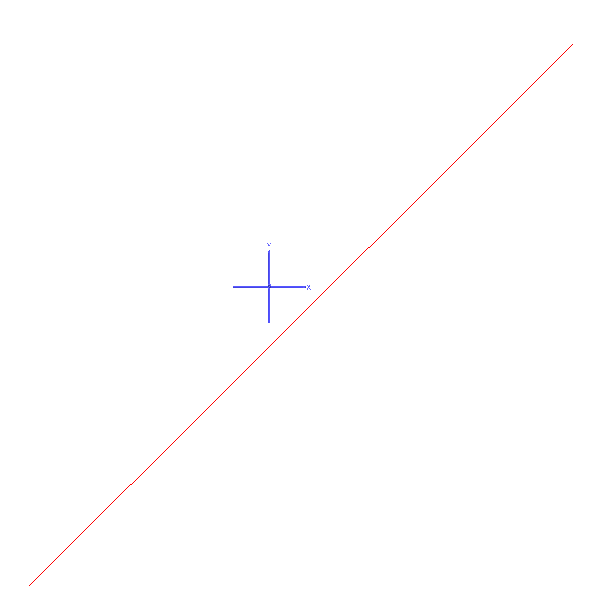
\includegraphics[width=.8\linewidth]{fig/1a2}
	  \caption{Resolution: 2}
	\end{subfigure}%
	\begin{subfigure}{.5\textwidth}
	  \centering
	  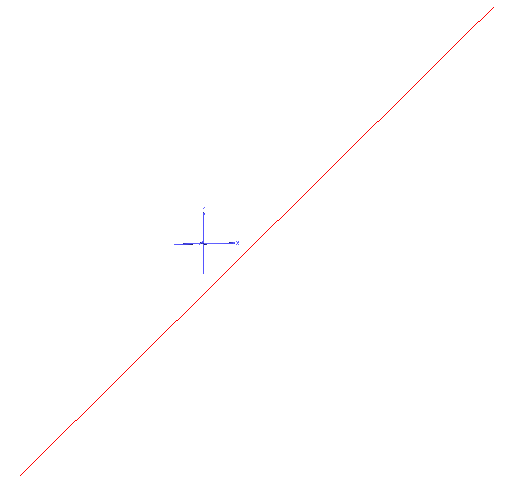
\includegraphics[width=.8\linewidth]{fig/1a100}
	  \caption{Resolution: 100}
	\end{subfigure}
	\caption{Plots of the straight line segment defined in "\textbf{1a.wrl}" with differing resolutions}
	\label{fig:1a}
\end{figure}

As seen in Fig. \ref{fig:1a} above, a sampling resolution of \textbf{2} is sufficient for drawing a straight line segement.

\subsection{Circular Arc}
\begin{figure}[H]
	\begin{subfigure}{.4\textwidth}
	  \centering
	  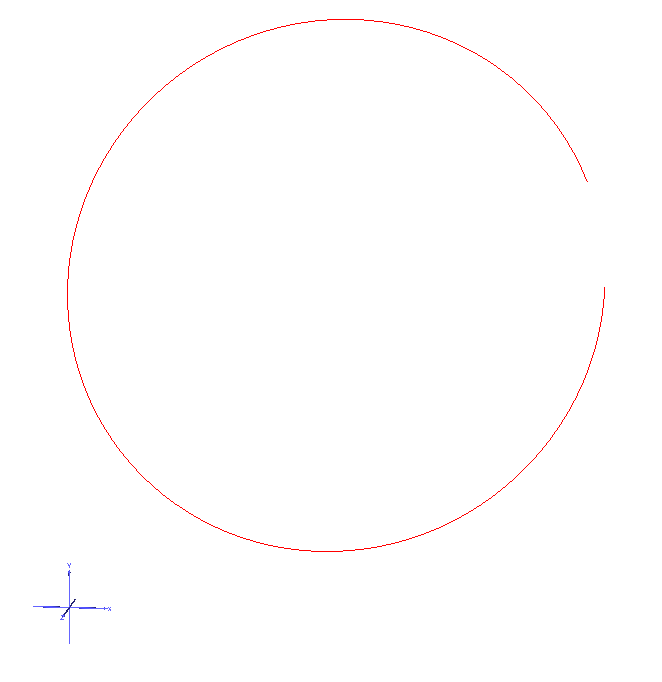
\includegraphics[width=.8\linewidth]{fig/1b120}
	  \caption{Resolution: 120}
	\end{subfigure}%
	\begin{subfigure}{.4\textwidth}
	  \centering
	  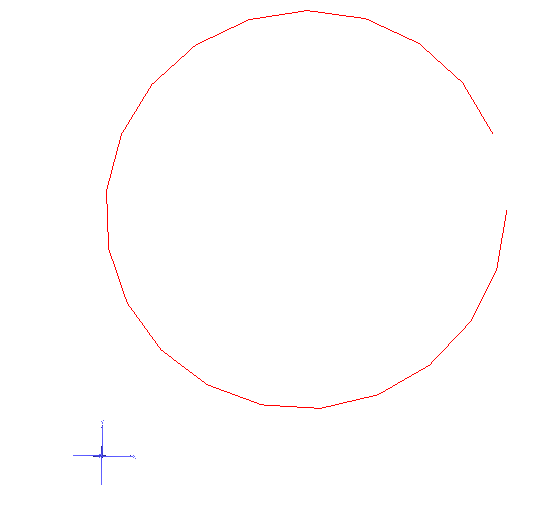
\includegraphics[width=.8\linewidth]{fig/1b20}
	  \caption{Resolution: 20}
	\end{subfigure}
	\caption{Plots of the circular arc segment defined in "\textbf{1b.wrl}" with differing resolutions}
	\label{fig:1b}
\end{figure}

As seen in Fig. \ref{fig:1b} above, a higher sampling resolution of \textbf{120} is required for drawing the circular arc in order for
it to appear as a smooth arc. When the sampling resolution is reduced to 20, the polyline interpolation of the curve is revealed.



\subsection{2D Spiral Curve}
\begin{figure}[H]
	\begin{subfigure}{.4\textwidth}
	  \centering
	  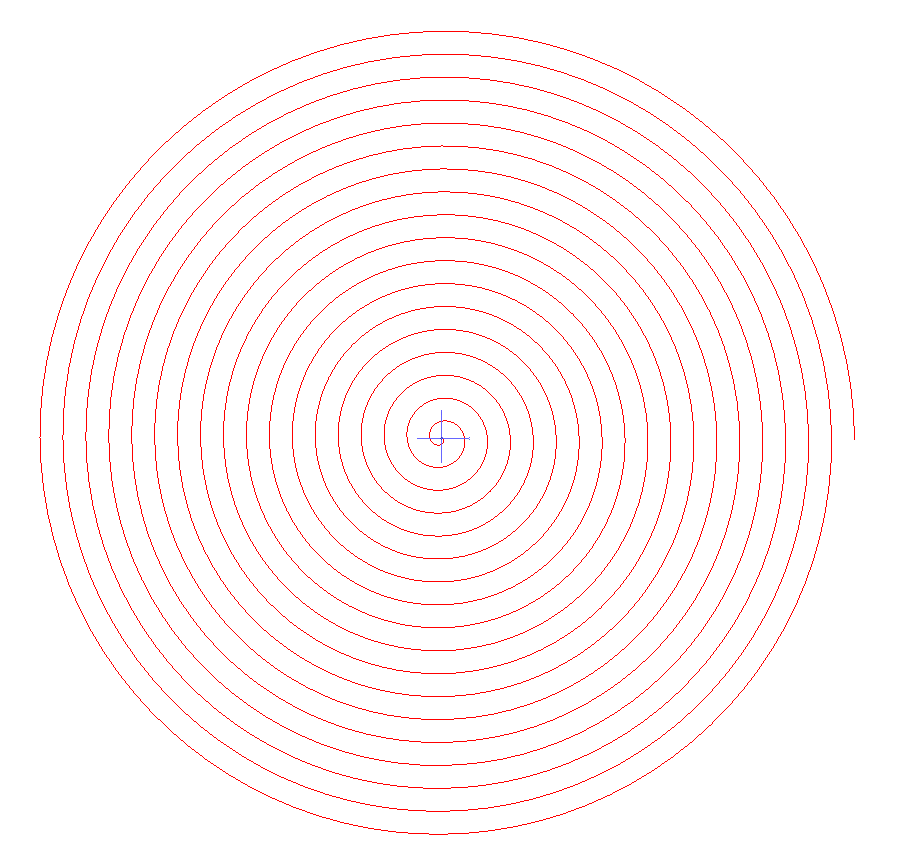
\includegraphics[width=.8\linewidth]{fig/1c1800}
	  \caption{Resolution: 1800}
	\end{subfigure}%
	\begin{subfigure}{.4\textwidth}
	  \centering
	  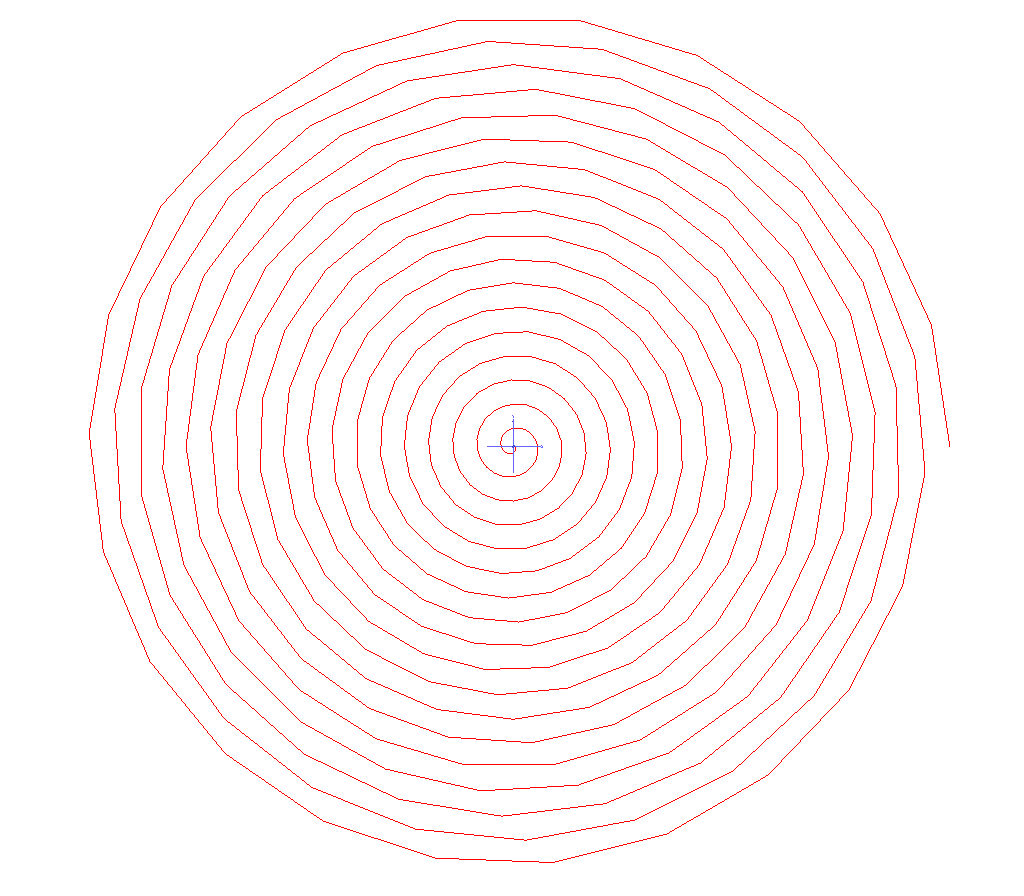
\includegraphics[width=.8\linewidth]{fig/1c400}
	  \caption{Resolution: 400}
	  \label{fig:1cb}
	\end{subfigure}
	\caption{Plots of the spiral curve defined in "\textbf{1c.wrl}" with differing resolutions}
	\label{fig:1c}
\end{figure}

As seen in Fig. \ref{fig:1c} above, a much higher sampling resolution of \textbf{1800} is required for drawing the spiral curve in order for
it to appear smooth. This is due to the fact that the spiral has a large number of spirals (18), and therefore the sampling 
locations on the outer part of the spiral are further apart as compared to the inner part of the spiral. 

This can be seen when the sampling resolution is reduced to 400 in Fig \ref{fig:1cb}, the inner parts of the spiral appears smooth, while 
the polyline interpolations can be seen on the outer parts of the spiral

\subsection{3D Cylindrical Helix}
\begin{figure}[H]
	\begin{subfigure}{.4\textwidth}
	  \centering
	  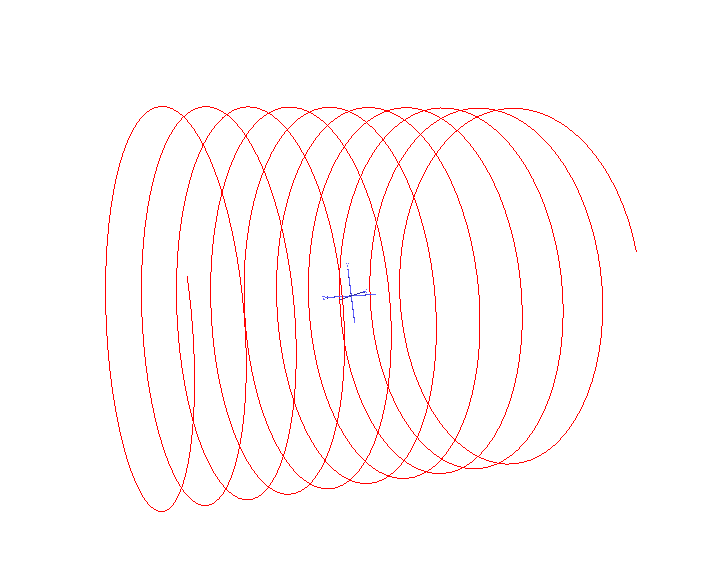
\includegraphics[width=.8\linewidth]{fig/1d800}
	  \caption{Resolution: 800}
	\end{subfigure}%
	\begin{subfigure}{.4\textwidth}
	  \centering
	  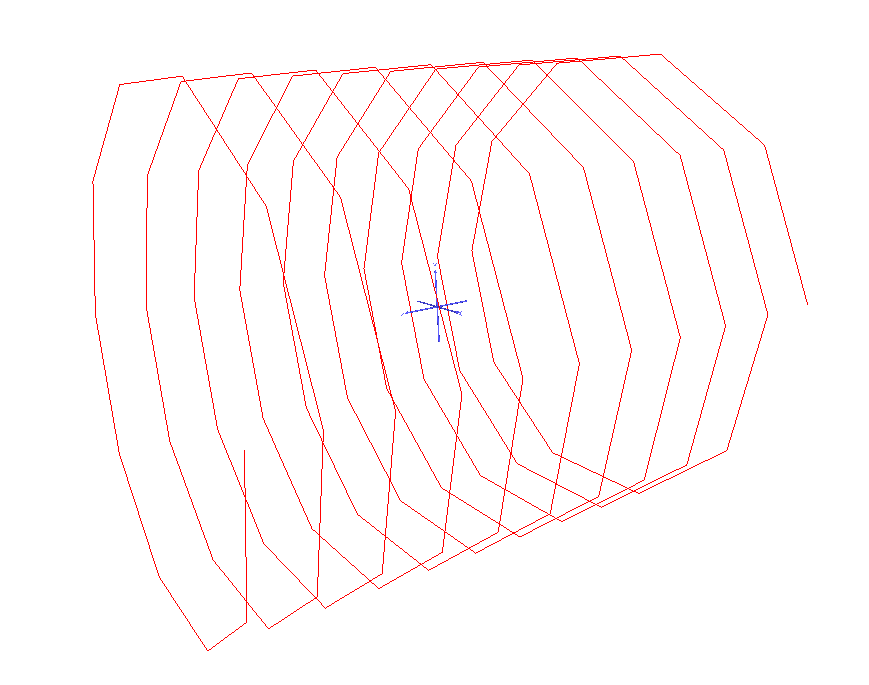
\includegraphics[width=.8\linewidth]{fig/1d100}
	  \caption{Resolution: 100}
	\end{subfigure}
	\caption{Plots of the cylindrical helix defined in "\textbf{1d.wrl}" with differing resolutions}
	\label{fig:1d}
\end{figure}

As seen in Fig. \ref{fig:1d} above, a much higher sampling resolution of \textbf{800} is required for drawing the cylindrical helix in order for
it to appear smooth. When the sampling resolution is reduced to 100, the polyline interpolation of the curve is revealed.

\pagebreak
\section{Converting Explicitly Defined Curve to Parametric Representations}
For this task, an explicitly defined curve has to be converted to its Parametric Representations. The following explicitly defined 
curve was assigned:

\begin{displaymath}
	y = tanh \ x
\end{displaymath}
\begin{displaymath}
	x \in [-1.3N, 2N], where \  N = 8
\end{displaymath}
\\Therefore, the follow parametric functions can be obtained:
\begin{displaymath}
	x(u) = (-1.3 * 8) + u * ((2+1.3) * 8)
\end{displaymath}
\begin{displaymath}
	\mathbf{x(u) = -10.4 + 26.4*u}
\end{displaymath}
\begin{displaymath}
	\mathbf{y(u) = tanh(-10.4 + 26.4*u)}
\end{displaymath}
\begin{displaymath}
	u \in [0,1]
\end{displaymath}
\\
By plotting the parametric equations defined above, we get the following display:
\begin{figure}[H]
	\centering
	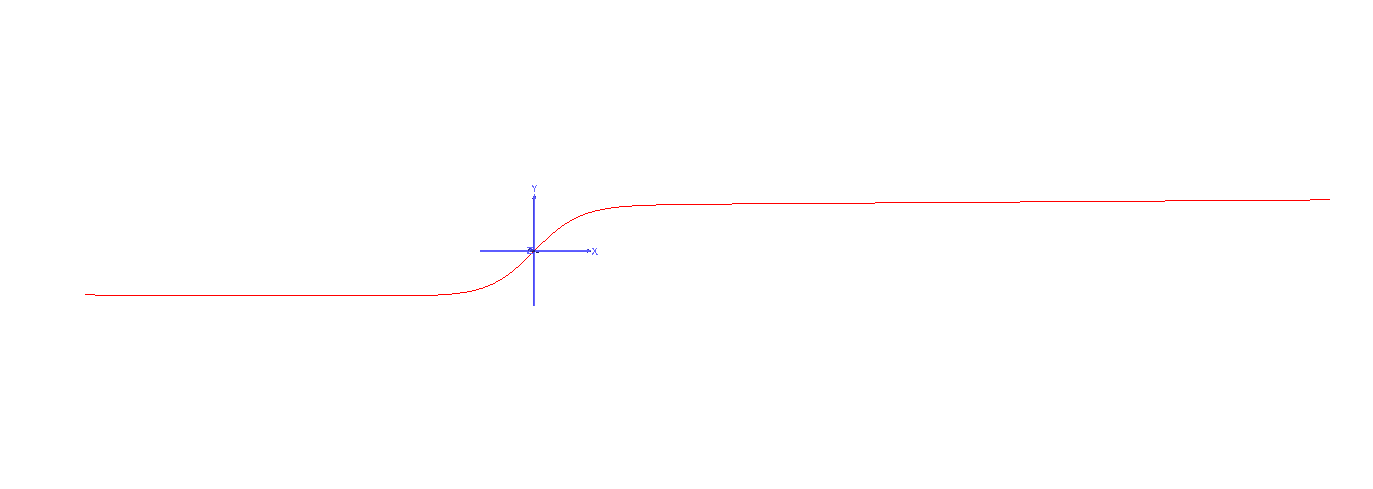
\includegraphics[width=.9\linewidth]{fig/2}
	\caption{Plot of the parametrically defined curve in "\textbf{2.wrl}"}
	\label{fig:2}
\end{figure}

\pagebreak
\section{Converting Curve Defined in Polar Coordinates to Parametric Representations}
For this task, a curve defined using polar coordinates has to be converted to its Parametric Representations. 
The curve is defined by:


\begin{displaymath}
	r = N - (M+5) cos \alpha \ \ \ \alpha \in [0, 2\pi],\ N = 8,\ M = 10
\end{displaymath}
\begin{displaymath}
	r = 8 - (10 + 5) cos(\alpha)
\end{displaymath}
\begin{displaymath}
	r = 8 - (15) cos(\alpha)
\end{displaymath}
\\We can convert between polar to cartesian with the following formulas:
\begin{displaymath}
	x = rcos(\alpha)
\end{displaymath}
\begin{displaymath}
	y = rsin(\alpha)
\end{displaymath}
\\Therefore, we can get:
\begin{displaymath}
	x(\alpha) =  (8 - 15cos(\alpha))cos(\alpha)
\end{displaymath}
\begin{displaymath}
	y(\alpha) =  (8 - 15cos(\alpha))sin(\alpha)
\end{displaymath}
\begin{displaymath}
	\alpha \in [0, 2\pi]
\end{displaymath}
\\Converting domain from \(\alpha\) to u:
\begin{displaymath}
	\mathbf{x(u) =  (8 - 15cos(2\pi u))cos(2\pi u)}
\end{displaymath}
\begin{displaymath}
	\mathbf{y(u) =  (8 - 15cos(2\pi u))sin(2\pi u)}
\end{displaymath}
\begin{displaymath}
	u \in [0, 1]
\end{displaymath}

By plotting the parametric equations defined above, we get the following display:
\begin{figure}[H]
	\centering
	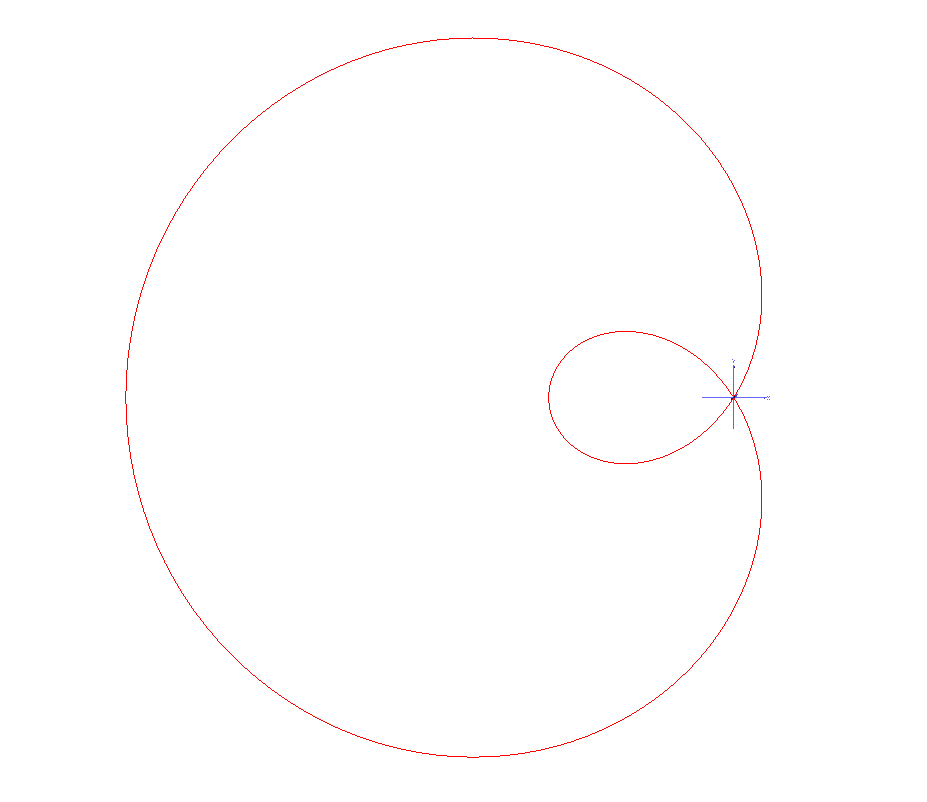
\includegraphics[width=.5\linewidth]{fig/3}
	\caption{Plot of the parametrically defined curve in "\textbf{3.wrl}"}
	\label{fig:3}
\end{figure}


% \begin{figure}[h]
% 	\centering
% 	\includegraphics[scale=0.47]{datasetfields}
% 	\caption{Dimensions and names of variables in the dataset}
% 	\label{fig:datasetfields}
% \end{figure}

%%
%% The acknowledgments section is defined using the "acks" environment
%% (and NOT an unnumbered section). This ensures the proper
%% identification of the section in the article metadata, and the
%% consistent spelling of the heading.


\bibliographystyle{ACM-Reference-Format}
\newpage





\end{document}
\endinput
%%
%% End of file `sample-acmlarge.tex'.
